 % Marco Metodologico.
\chapter{Marco Metodológico} \label{chap:Marco Metodologico}

\vspace{5 mm}

En este capítulo se describe la metodología utilizada para el desarrollo del proyecto, la cual es una versión “ágil” de OpenUp y se denomina Metodología de Proyectos Synergy-GB; además, se describe brevemente el marco de trabajo utilizado para la gestión del desarrollo del prototipo funcional tanto de la aplicación web como de la aplicación móvil de Notificaciones+.


Para efectos de este proyecto de pasantía, son muchos los artefactos que se describen en la Metodología de Proyectos Synergy-GB que no son aplicables al mismo ya que consisten en entregables directos a algún cliente, y en este caso el cliente es la misma empresa.


\section{Metodología de Proyectos Synergy-GB} \label{sect:Metodologia Synergy}
Describe las herramientas y artefactos que facilitan la comunicación y alineación tanto interna  (entre los integrantes del equipo de trabajo) como externa (de Synergy-GB hacia el cliente) en cuanto al seguimiento y progreso de los proyectos \cite{MMSynergy}. 

En la Figura ~\ref{fig:metosyn} se muestran las etapas en las cuales de divide la Metodología de Proyectos Synergy-GB \cite{MMSynergy}.

\begin{figure}
  \centering
  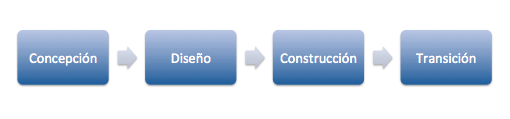
\includegraphics[scale=0.7,type=png,ext=.png,read=.png,angle=0,origin=c]{imagenes/metodologiasynergy}
  \caption{Etapas de la Metodología de Proyectos Synergy-GB. 
(Synergy-GB Área de Calidad).}
  \label{fig:metosyn}
\end{figure}

\subsection{Concepción}
En esta etapa se definen los documentos de requerimientos y el acuerdo con el cliente, acerca de los entregables que se deben realizar en el proceso de ejecución del proyecto. Los involucrados en esta etapa son el líder de proyecto (Synergy-GB) y el cliente, y la persona responsable de cada una de las actividades es el líder de proyecto \cite{MMSynergy}.

\subsection{Diseño}
En esta etapa se construyen los diseños de funcionalidad y servicios que se requieren para la etapa de construcción del producto. Las personas involucradas en esta etapa de la metodología son: líder de proyecto, arquitecto, diseñador, integración y calidad \cite{MMSynergy}.

\subsection{Construcción}
En esta etapa del proyecto, se realiza el desarrollo de la aplicación por parte del equipo del proyecto (Integración, Ux, Móvil, Web) encargado en el área correspondiente; en este caso, el encargado designado por la empresa es el pasante. Para su gestión, se utilizó el marco de trabajo Scrum. La fase de dividió en tres (3) iteraciones, de un mes de duración cada una. En el capítulo 5 se describirá con más detalle las actividades realizadas \cite{MMSynergy}.

\subsection{Transición}
La etapa de transición representa un punto de validación y cierre para el proyecto. Es en este momento cuando se realizan todas las pruebas sobre los distintos componentes de la solución, determinando que su funcionamiento es el correcto y su presentación cumple con los diseños elaborados en tempranas etapas. Por lo tanto,  se llevan a cabo las pruebas de estrés por parte del equipo de Integración y Ux, y luego las pruebas de los servicios e integrales por parte del equipo de calidad involucrado en el proyecto \cite{MMSynergy}.

\section{Scrum} \label{sect:Scrum}
Es un marco de trabajo dentro del cual las personas pueden  afrontar complejos problemas adaptativos, a la vez que entregan productos del máximo valor posible de forma proactiva y creativa. No es una técnica de construcción de productos, sino simplemente un marco de trabajo flexible en donde se pueden emplear diversas técnicas o procesos \cite{MMSCRM}. 

Scrum se fundamenta en la teoría empírica de procesos, en donde se asegura que el conocimiento procede de la experiencia y de tomar decisiones basándose en lo que se conoce. Scrum emplea una aproximación iterativa e incremental para optimizar la predictibilidad y controlar el riesgo \cite{MMSCRM}.

Al fundamentarse en la teoría empírica de procesos, Scrum debe soportarse sobre los siguientes tres pilares: transparencia, inspección y adaptación \cite{MMSCRM}.

\subsection{El equipo Scrum (Scrum team)}
El Scrum team está conformado por el dueño del producto, el equipo de desarrollo y el Scrum master (jefe del Scrum o facilitador). A continuación, se especifican las responsabilidades de cada uno de los integrantes del equipo \cite{MMSCRM}:

\begin{itemize}[noitemsep,nolistsep]
\item {Dueño del producto (product owner):}

Es el encargado de maximizar el valor del producto y del trabajo del equipo de desarrollo; a su vez, es la única persona que puede gestionar el product backlog (pila del  producto, más adelante se especificará qué es exactamente). Es el responsable del producto desde un punto de vista comercial o de negocio.
\item {Equipo de desarrollo:}

Es el equipo de trabajo que participa en un Sprint dentro de la práctica Scrum. Realiza las tareas de diseño y desarrollo de \textit{software}. Desde un punto de vista más general, son los profesionales que realizan los incrementos de un producto, posiblemente funcional, al final de cada sprint. Sólo los integrantes del equipo de desarrollo están autorizados para realizar los incrementos del producto.
\item {Scrum master:}

Tiene como responsabilidad asegurar que Scrum, como marco de trabajo, es entendido y llevado a cabo correctamente. Es un líder servil que se encuentra a la orden de todo el Scrum team. Por otra parte, el Scrum master es aquel puente entre agentes externos al Scrum team y este último.
\end{itemize}

\subsection{El Sprint}
El núcleo de Scrum es el Sprint, un período de tiempo de a lo sumo un mes durante el cual se crea un incremento de producto utilizable y potencialmente entregable. Cada nuevo sprint comienza inmediatamente después de la finalización del Sprint anterior \cite{MMSCRM}.

Para asegurar el correcto funcionamiento del sprint, deben seguirse las siguientes normas \cite{MMSCRM}:
\begin{itemize}[noitemsep,nolistsep]
\item No se realizan cambios que afectarían al objetivo del sprint.
\item La composición del Equipo de Desarrollo se mantiene constante.
\item	Los objetivos de calidad no disminuyen.
\item	El alcance puede ser clarificado y renegociado entre el Dueño de Producto y el Equipo de Desarrollo a medida que se va aprendiendo más.
\end{itemize}

Los Sprints están compuestos por la reunión de planificación del sprint (Sprint Planning Meeting), los Scrums diarios (Daily Scrums), el trabajo de desarrollo, la revisión del sprint (Sprint review), y la retrospectiva del sprint (Sprint Retrospective) \cite{MMSCRM}:

\begin{itemize}[noitemsep,nolistsep]
\item {Reunión de Planificación del Sprint (Sprint Planning Meeting):}

El trabajo a realizar durante el Sprint es planificado en la Reunión de Planificación de Sprint. Este plan es creado mediante el trabajo colaborativo del Equipo Scrum al completo.
La Reunión de Planificación de Sprint consta de dos partes, cada una de ellas da respuesta a las siguientes preguntas, respectivamente: ¿Qué será entregado en el Incremento resultante del Sprint que comienza? ¿Cómo se conseguirá hacer el trabajo necesario para conseguir el Incremento?
\item {Scrum Diarios (Daily Scrums):}

Es una reunión de máximo 15 minutos, para que el Equipo de Desarrollo sincronice sus actividades y cree un plan para las siguientes 24 horas. Esto se lleva a cabo inspeccionando el trabajo avanzado desde el último Scrum Diario y haciendo una predicción acerca del trabajo que podría ser completado antes del siguiente. 
\item {Revisión del Sprint (Sprint Review):}

Al final del Sprint se lleva a cabo una Revisión de Sprint, para inspeccionar el Incremento y adaptar la Pila de Producto si fuese necesario. Durante la Revisión de Sprint, el Equipo Scrum y los interesados colaboran acerca de lo que se ha hecho durante el Sprint.
\item {Retrospectiva del Sprint (Sprint Retrospective):}

La Retrospectiva de Sprint es una oportunidad para el Equipo Scrum de inspeccionarse a sí mismo, y crear un plan de mejoras que sean abordadas durante el siguiente Sprint.
\end{itemize}

\subsection{Artefactos}
Los artefactos de Scrum representan trabajo o valor en diversas formas que son útiles para proporcionar transparencia y oportunidades para la inspección y adaptación. Los artefactos definidos por Scrum, están específicamente diseñados para maximizar la transparencia de la información clave, que es necesaria para asegurar que los Equipos Scrum tengan éxito al entregar un Incremento \cite{MMSCRM}:
\begin{itemize}[noitemsep,nolistsep]
\item {Pila de Producto (Product Backlog):}

La Pila de Producto es una lista ordenada de todo lo que podría ser necesario en el producto, y es la única fuente de requerimientos para cualquier cambio a  realizarse en el producto. El Dueño de Producto (Product Owner) es el responsable de la Pila de Producto, incluyendo su contenido, disponibilidad y ordenación.
\item {Pila de Sprint (Sprint Backlog):}

La Pila de Sprint es el conjunto de elementos de la Pila de Producto seleccionados para el Sprint, más un plan para entregar el Incremento de producto y conseguir el Objetivo del Sprint. \\
\end{itemize}
Para los efectos de esta pasantía, el dueño del producto fue Alexander Ramírez. El scrum master fue Ana Dávila y el desarrollador fue el pasante designado por la empresa, supervisado por el líder del área de movilidad Gabriel Vega.

Se desarrollaron los siguientes documentos entregables desde el punto de vista de un proyecto de \textit{software}, los cuales a su vez, representan la documentación del sistema obtenido como resultado de la pasantía: Documento de Arquitectura de Software y Documento de Especificación Funcional.
